\label{desenvolvimento}

Neste Capítulo será apresentada a segunda fase do \textit{Design Science Research} -- Sugestão -- onde serão exploradas: a proposta do guia; como ele será trabalhado; como foi realizado o desenvolvimento da ferramenta; como é a interface que será apresentada ao usuário; a forma de se utilizar os \textit{cards} no sistema; e como eles podem ser editados para adequações futuras em outras propostas de ferramentas para elicitação de requisitos éticos em \acrshort{IA}.

\section{Proposta}

A ferramenta proposta neste trabalho servirá como um assistente para os \textit{Product Owners} e desenvolvedores elicitarem requisitos éticos em sistemas baseados em IA durante a primeira fase do ciclo de desenvolvimento de software (i.e., a análise de requisitos), no contexto de desenvolvimento ágil de software. Para esta fase de discussão, será utilizado um formato de \textit{Planning Poker} digital, com acesso disponível \href{https://oggvaldo.GitHub.io/eccola}{no repositório no GitHub}.

Será implementado um método desenvolvido por Vakkuri et al. \cite{ECCOLA} denominado ECCOLA, onde os autores conceberam um baralho de \textit{cards} com questões éticas a serem debatidas pela a equipe de desenvolvimento. A implementação dos \textit{cards} de papel em uma interface gráfica se justifica no contexto de trabalho remoto devido a pandemia do COVID-19, além de prover um meio adequado para que pesquisadores possam avaliar a ferramenta de maneira mais automatizada. O modelo adotado de \textit{Planning Poker} propõe uma discussão de forma mais lúdico, de fácil entendimento e praticidade, uma vez que a ferramenta poderá ser acessada tanto por dispositivos móveis (\textit{smartphones} e \textit{tablets}) quanto computadores (\textit{desktops} e \textit{notebooks}).

\section{Desenvolvimento}

Para o desenvolvimento deste sistema, foram utilizadas as tecnologias de \textit{Hypertext Markup Language} \acrshort{HTML} \cite{HTMLsite}, \textit{Cascading Style Sheets} \acrshort{CSS} \cite{CSSsite} e JavaScript \acrshort{JS} \cite{JavaScriptsite}. Para a apresentação da página inicial e a página que vai apresentar os \textit{cards}, temos o \acrshort{HTML} como a base, o \acrshort{CSS} como a parte de estilização da página, além de fornecer padrões adaptativos para diversos tamanhos de tela, manutenabilidade e escalabilidade visual do programa sem a necessidade de ferramentas e \textit{frameworks} adicionais, e o \acrshort{JS} como a parte responsável pela lógica e ação de funcionalidades do sistema. Com este conjunto de ações, teremos aqui o que será um tipo de aplicação web, uma aplicação que funcionará diretamente do navegador de qualquer dispositivo com capacidade computacional e que seja compatível com \acrshort{HTML} 5 \cite{webapp}.

Com isso, temos um sistema totalmente responsivo a diversos tamanhos de tela. Isto permite seu uso em dispositivos como \textit{smartphones}, \textit{tablets}, \textit{notebooks} e computadores de mesa. Temos esta possibilidade devido o emprego de \textit{Media Queries} do \acrshort{CSS} empregado, que viabiliza a realização da apresentação do conteúdo de forma adaptativa a cada um dos dispositivos supracitados, sem a necessidade de se realizar alterações específicas para cada um dos tipos de equipamentos e/ou telas.

Durante a criação deste guia, alguns cuidados foram tomados. O \acrshort{HTML} foi criado de forma a permitir a legibilidade e compreensibilidade com o uso devido do \acrshort{HTML} semântico (por exemplo, como as tags semânticas identificam o conteúdo que se encontra nos arquivos do sistema), permitindo assim a leitura do código de forma mais sucinta e de mais fácil identificação. Além disto, o sistema foi projetado também de forma a ser utilizada por pessoas com deficiência visual devido ao emprego de tal técnica. Para tanto, este sistema está satisfatoriamente adaptado ao uso de sistemas ledores de tela, como o \href{https://www.nvaccess.org/}{\textit{Non Visual Desktop Access} (NVDA)}.

Simultaneamente com a disponibilização do site estático com o uso do \acrshort{HTML} e do \acrshort{CSS}, o \acrshort{JS} foi utilizado para trazer ao sistema os elementos que fornecem a interatividade e o dinamismo do sistema para os usuários. Assim, foi possível dar ao usuário as possibilidades de seleção e comparação dos \textit{cards}, filtragem de acordo o princípio ético que pretendem explorar e a facilidade na realização de alterações do sistema para outros tipos de elicitações a serem inseridos no sistema, permitindo desta maneira, a futuros desenvolvedores a possibilidade de modificar e adicionar \textit{cards} e princípios éticos com baixa complexidade, objetivando um sistema com a qualidade de \textit{user-friendly}, tanto para quem irá operar (e.g., Product Owners, desenvolvedores de sistemas baseados em IA) quanto para quem irá editar o sistema (e.g., pesquisadores de ética em IA) através do acesso aberto ao código do sistema no repositório localizado no  \href{https://www.GitHub.com/oggvaldo/eccola}{repositório}, onde a fonte se encontra disponível.

Com isso, temos em mente o objetivo de contemplar os princípios éticos encontrados na área de ética em IA com o fornecimento do sistema e de seu código-fonte, compreensibilidade e instruções de uso explorando o princípio ético da transparência, com foco nas questões éticas de divulgação, comunicação, apresentação, explicabilidade, compreensibilidade e interpretabilidade, e ao adequar a tecnologia para o uso de \textit{softwares} leitores de tela temos a contemplação do princípio de beneficência e dignidade atendidos segundo os princípios éticos definidos por Ryan e Stahl \cite{Ryan2020ArtificialIE}.

Com todos os aspectos técnicos de software descritos anteriormente, na entrada do sistema o usuário poderá ler como se utiliza os \textit{cards} em um contexto de desenvolvimento ágil com o uso da técnica de \textit{Planning Poker}, conforme a figuras abaixo apresentam.

\begin{figure}[h!]
    \centering
    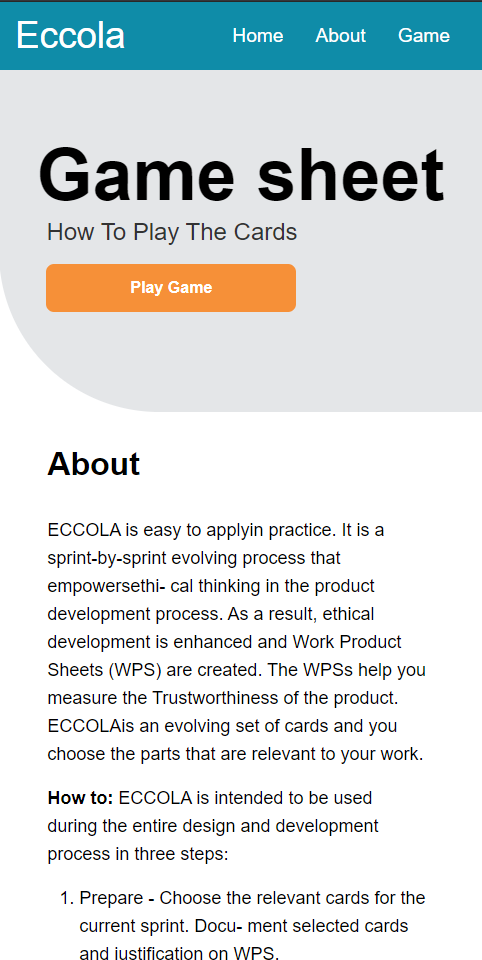
\includegraphics[width=0.5\textwidth]{img/eccola_celular.png}
    \caption{Imagem do sistema adaptado para telas de \textit{smartphones} e \textit{tablets}}
    \label{fig:eccola_celular}
\end{figure}

\begin{figure}[h!]
    \centering
    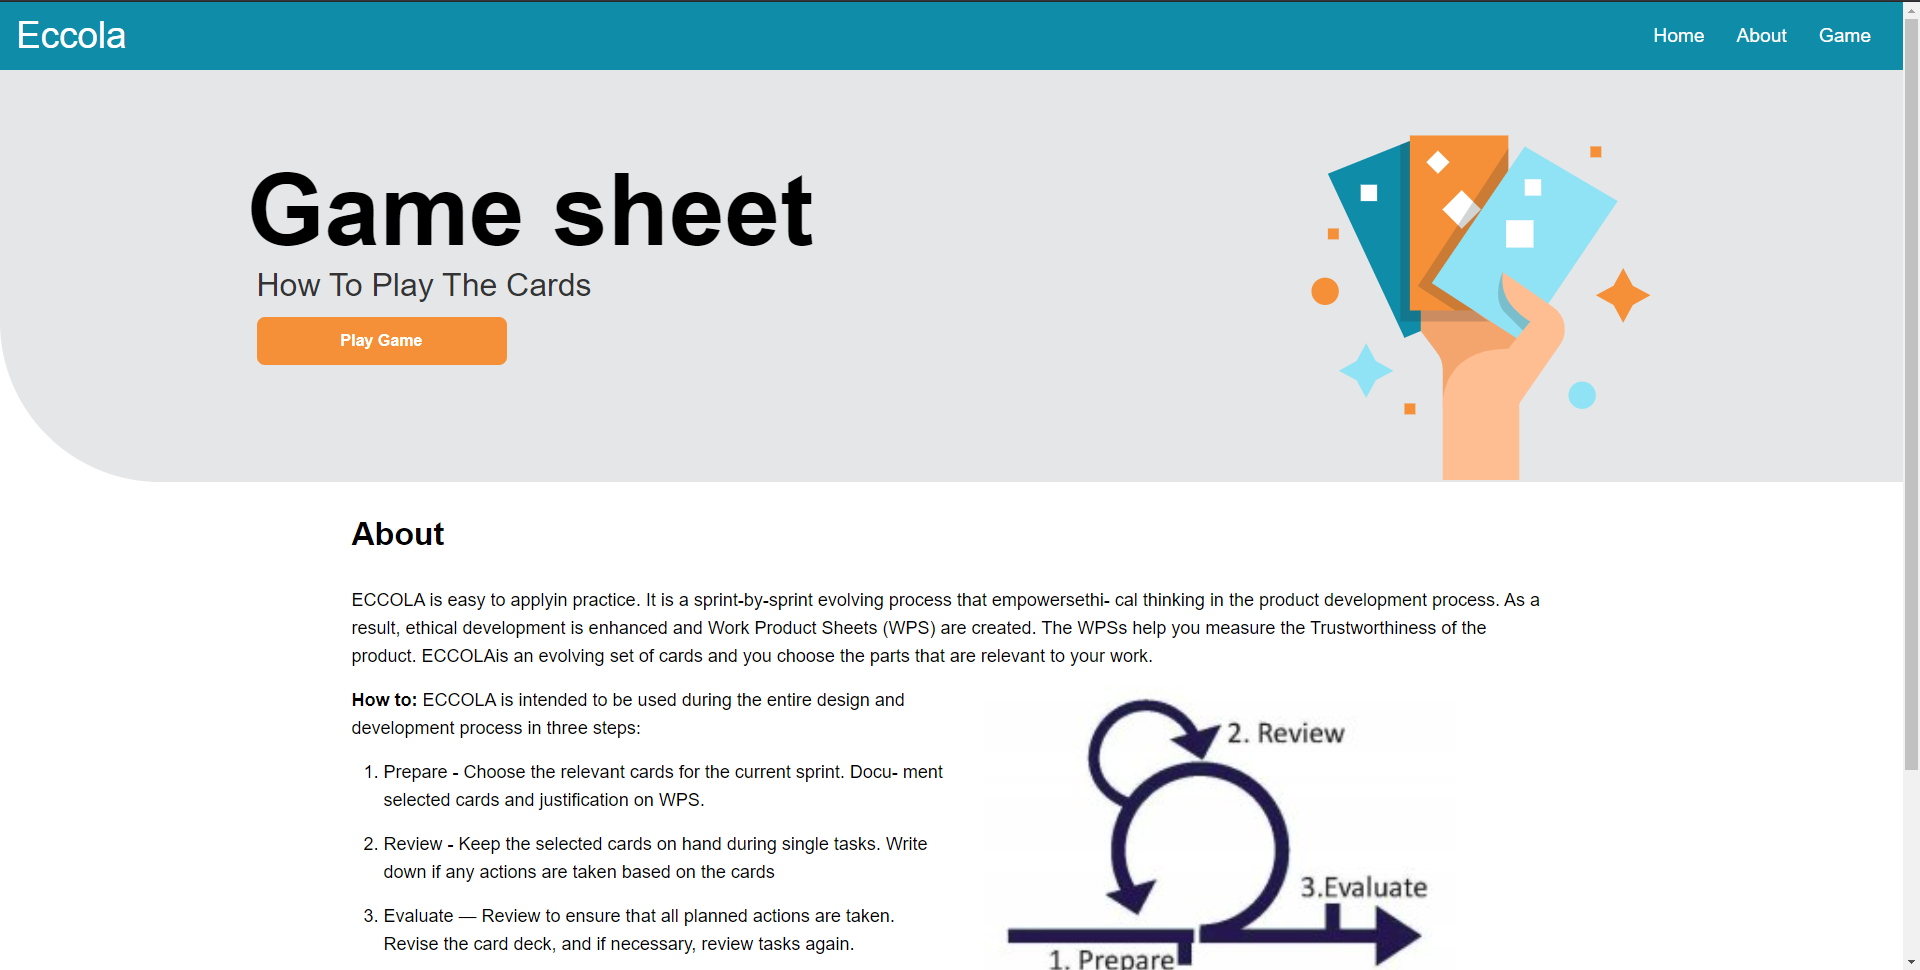
\includegraphics[width=\textwidth]{img/eccola_desktop.png}
    \caption{Imagem do sistema adaptado para telas de computadores de mesa e \textit{notebooks}.}
    \label{fig:eccola_desktop}
\end{figure}

\subsection{Interface}

Para a criação deste guia, a partir da inspiração de um \textit{Planning Poker} voltado para o debate de projetos, foi concebido que o sistema deveria apresentar seus tópicos através do formato de cards. Para tanto, vendo como o ECCOLA \cite{ECCOLA} fez a implantação em forma analógica (\textit{cards} físicos) do modelo e o mesmo pode ser aplicado para qualquer outro conjunto de regras de elicitação de requisitos de ética em \acrshort{IA}, foi julgado que adotar o modelo de \textit{cards} para a criação deste guia seria ainda o ideal.

Para tanto, usamos a plataforma de desenvolvimento de protótipos \href{https://www.figma.com/}{FIGMA}, no qual foi possível desenhar como seria o formato do guia e, a partir dele, criar um \textit{mockup} do que viria a ser o guia. Após a realização de um \textit{brainstorm} sobre como desenvolver o projeto, foi entendido que era necessário que o sistema apresentasse ao menos três telas, sendo uma de boas vindas do sistema, apresentando as regras do jogo, o que é e o título do sistema, uma com os \textit{cards} a serem mostrados aos participantes do planejamento e a tela onde se apresentam os \textit{cards} selecionadas apenas, com a opção de retorno e selecionar novamente os \textit{cards}. Ao término do projeto de prototipação, chegamos no desenho atual do guia, que pode ser acessado clicando \href{https://www.figma.com/file/zW8ISzBYMcIZFk6BoXZD4n/Eccola}{aqui}.

Com fortes inspirações nos modelos utilizados pelo design gráfico criado pelo Google, o Material Design influenciou fortemente na criação da interface dos \textit{cards}, ajudando-nos a adotar um modelo de \textit{card} que pudesse ser facilmente replicado e identificado, sem perder a característica de um visual limpo, informativo e agradável visualmente, independente da plataforma ao qual o guia esteja sendo utilizado. 

\begin{figure}[h!]
    \centering
    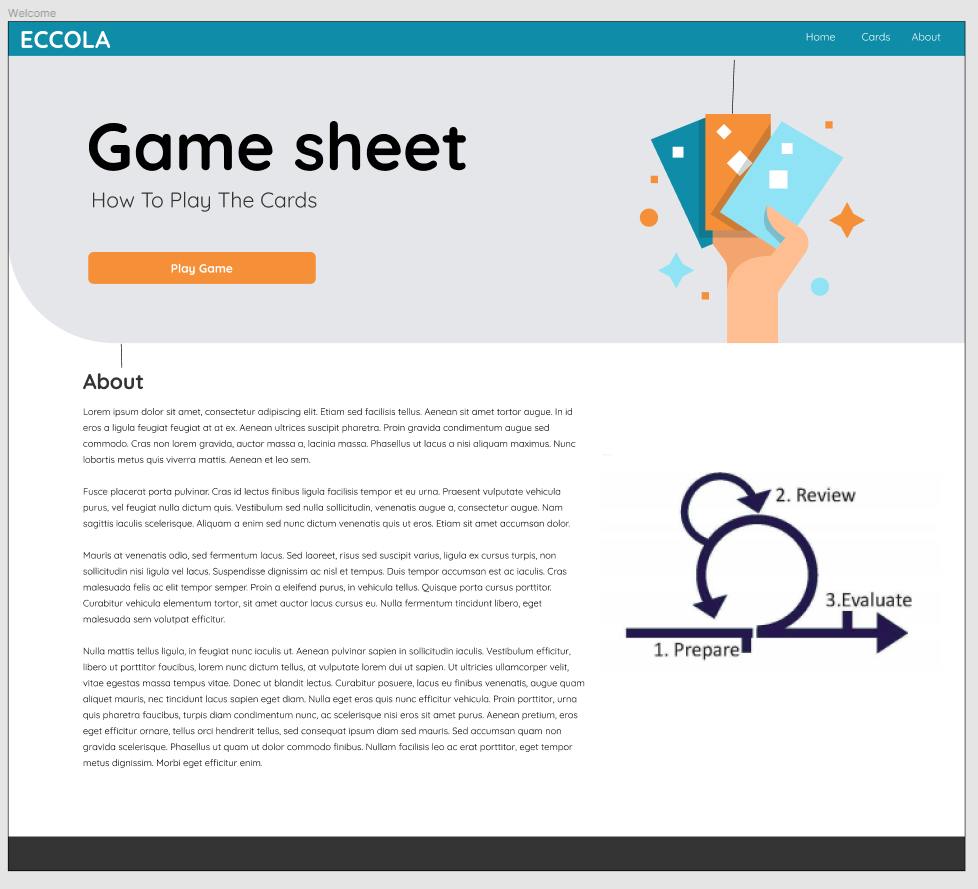
\includegraphics[width=\textwidth]{img/figma_welcome.png}
    \caption{Imagem do protótipo do sistema na tela inicial criado na ferramenta Figma.}
    \label{fig:figma_welcome}
\end{figure}

Para a tela de boas vindas, um design com poucas distrações, uma descrição de como se utilizar o sistema e a possibilidade de se inserir um arquivo mostrando como se trabalhar com os \textit{cards} (uma vez que estas são pensadas para serem utilizadas em projetos variados de elicitação de requisitos) ou outras descrições. Para tanto, basta que um usuário com conhecimentos em \acrshort{HTML} altere a página inicial ao seu gosto, de acordo as necessidades criadas pelo projeto a ser utilizado junto ao guia.

\begin{figure}[h!]
    \centering
    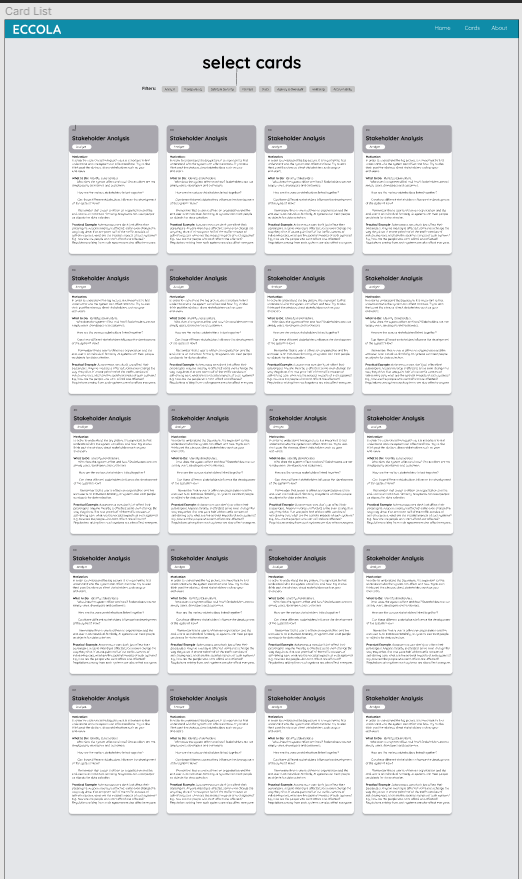
\includegraphics[width=0.7\textwidth]{img/figma_cards.png}
    \caption{Imagem do protótipo do sistema na tela de seleção de \textit{cards} criado na ferramenta Figma.}
    \label{fig:figma_cards}
\end{figure}

Para a tela de escolha dos cards, temos todos os \textit{cards} apresentados, com um menu \textit{drop-down} para o filtro de seleção da categoria dos \textit{cards} a serem escolhidas para a rodada de debate. Estos \textit{cards} e suas categorizações serão melhor detalhadas na seção \ref{Utilizando os cards}. Temos também o botão \textit{Compare cards}, onde após a seleção dos itens para o debate teremos o prosseguimento para a tela de resultados após apertar no botão.

\begin{figure}[h!]
    \centering
    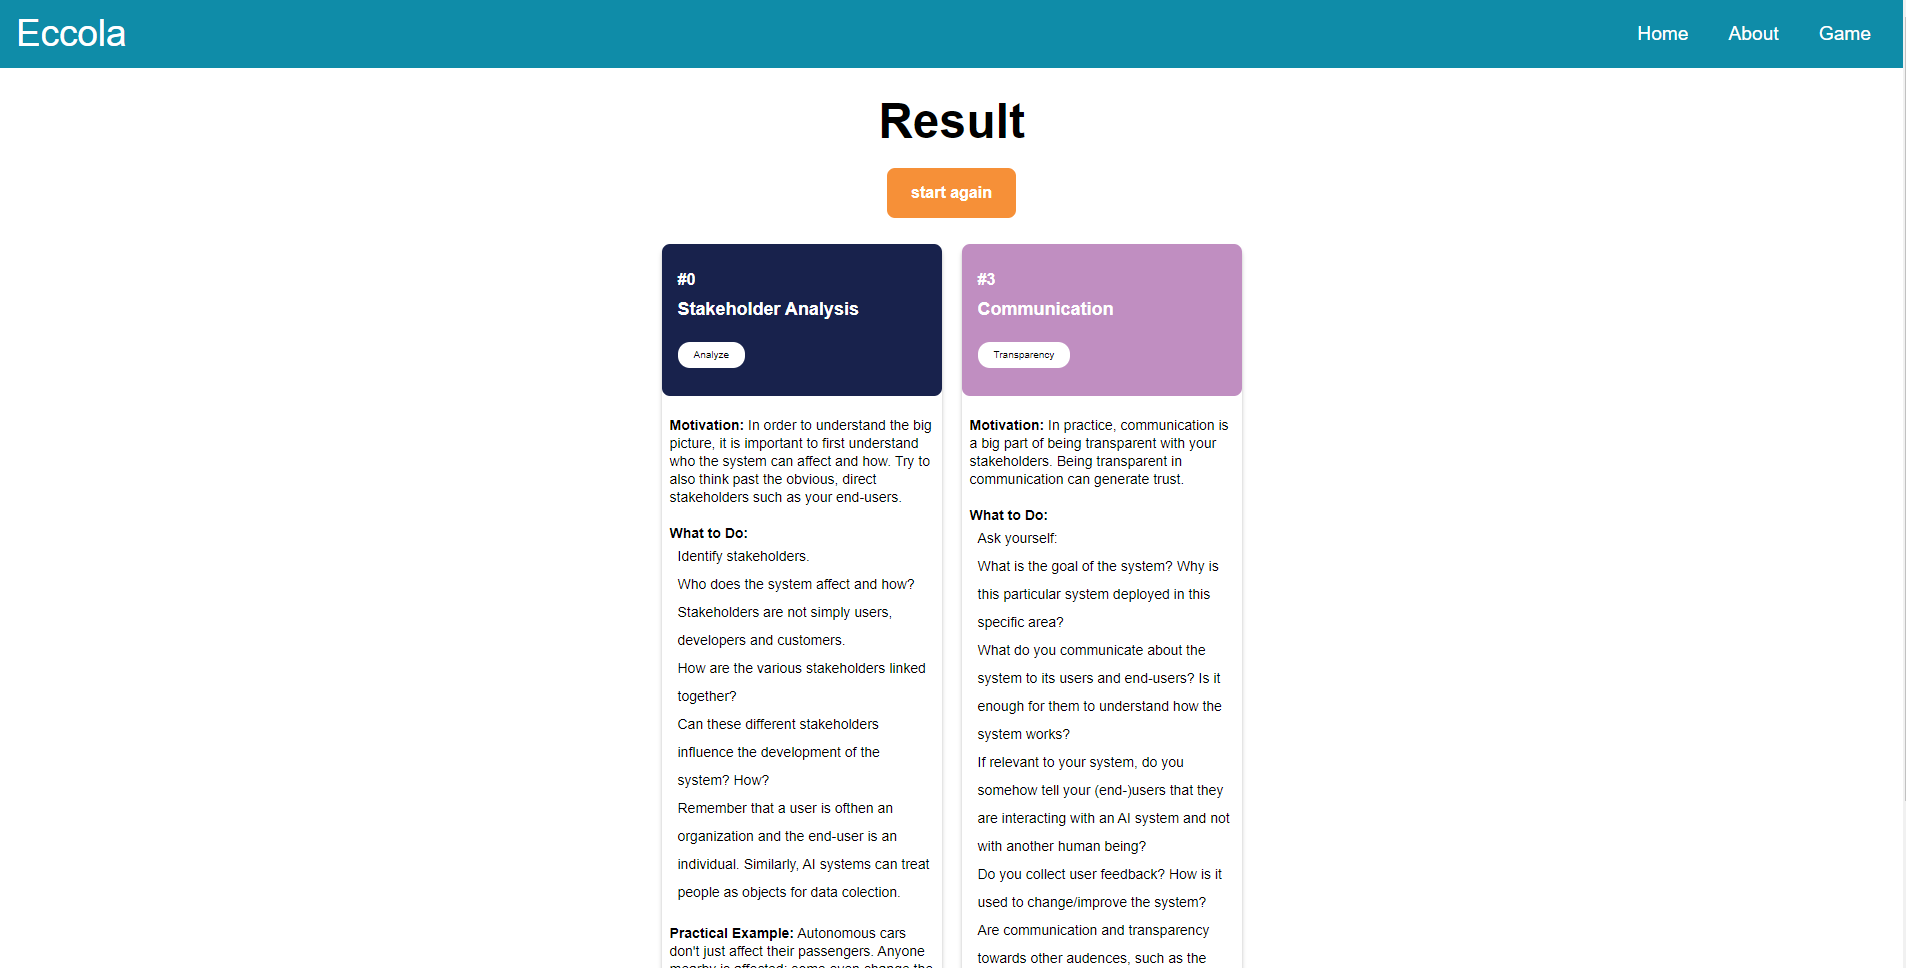
\includegraphics[width=\textwidth]{img/eccola_results.png}
    \caption{Imagem do sistema na tela de \textit{cards} selecionados.}
    \label{fig:eccola_results}
\end{figure}

Para a tela de resultados, durante a prototipação foi deixada a tela propositalmente em branco, porém na versão atual do sistema temos a apresentação dos \textit{cards} selecionadas na tela anterior juntamente com o botão \textit{Start again}, que permite, caso queira, realizar uma nova seleção dos itens para o debate, o que será abordado em maiores detalhes na Seção \ref{Como utilizar}.

\section{Como utilizar}
\label{Como utilizar}

Tomando como referência o ECCOLA, apresentado na Figura \ref{fig:eccola_desktop}, o sistema terá a tela inicial apresentando tanto um botão ``Play game'', seja no topo da tela ou ao final (inclusive no modo para dispositivos móveis) e os links Home, About e Game no topo da tela, onde cada um dos links envia para uma das páginas (as quais podem ser customizadas e serão detalhadas em maior profundidade na Seção \ref{editandocards}) citadas. Neste caso, o link \textit{Home} encaminha para a página inicial, o link \textit{About} para o espaço onde está a descrição do jogo a ser inserida e o link \textit{Game} para a página onde se encontram os \textit{cards}. O botão \textit{Play the Game} localizadas tanto no início quanto final da página  tem o mesmo propósito do link \textit{Game}, levando também para a página onde o \textit{Planning Poker} será realizado.

Na interface do \textit{Planning Poker}, como mostrado na figura \ref{fig:eccola_cards}, temos um menu \textit{dropdown} que serve como filtro, onde somente os \textit{cards} do tipo selecionado estarão sendo exibidas na tela caso o filtro \textit{ALL} não esteja ativo, o botão \textit{Compare Cards}, que será acionado somente em caso de selecionar dois \textit{cards} para a discussão (onde o número de \textit{cards} também pode ser alterado, como veremos adiante) e logo abaixo os \textit{cards} que estarão disponíveis para a seleção e discussão. Ao clicar em cada um dos cards, eles terão uma borda laranja ao selecionar os mesmos, onde após clicar no botão \textit{Compare Cards} teremos a tela mostrando apenas os \textit{cards} selecionados. Estes serão os \textit{cards} a serem utilizados no debate, e será apresentado como utilizá-los na Seção \ref{utilizandocards}.

\begin{figure}[h!]
    \centering
    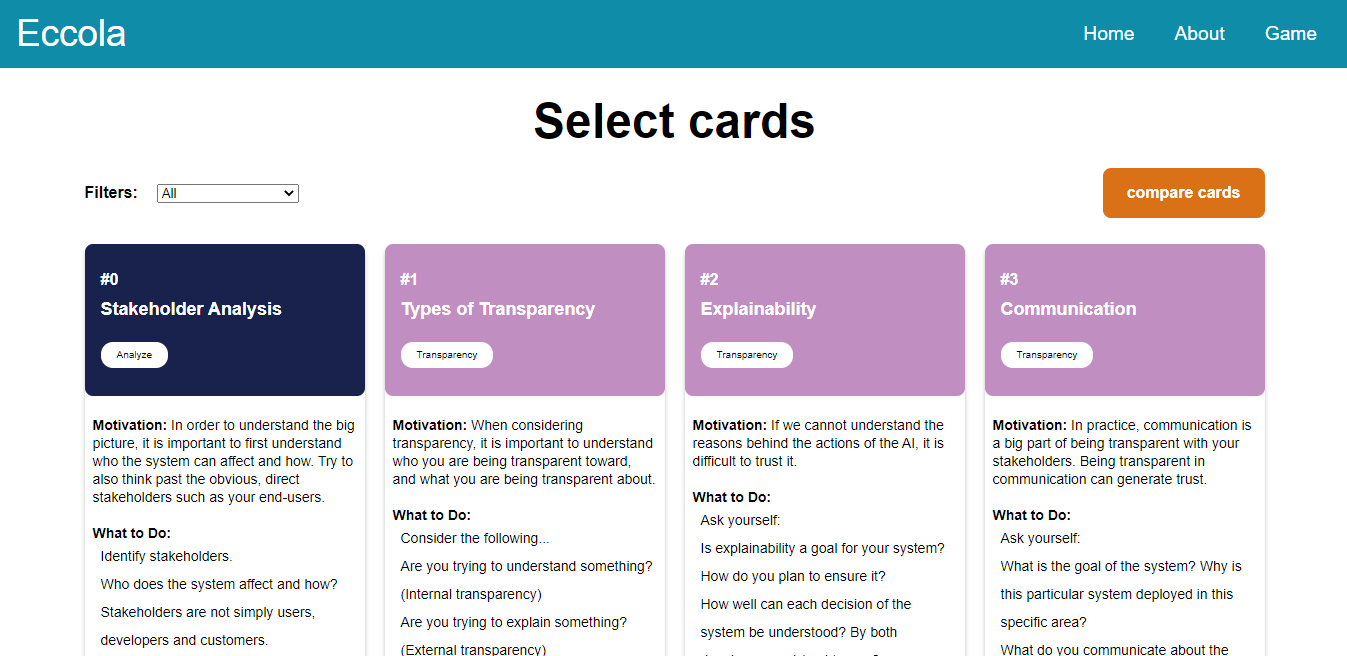
\includegraphics[width=\textwidth]{img/eccola_cards.png}
    \caption{Imagem do sistema com os \textit{cards} disponíveis em uma tela com resolução maior que 640 pixels.}
    \label{fig:eccola_cards}
\end{figure}

\subsection{Utilizando os \textit{cards}}
\label{utilizandocards}
Para a utilização do sistema, é necessário retomarmos aos conceitos de um \textit{Planning Poker} e adaptarmos ao uso no contexto de ética em IA. Para um melhor entendimento, temos que também adaptar o debate ao ambiente de desenvolvimento ágil e o uso do Scrum, já que sem estas ferramentas o uso deste guia fica muito mais limitado.

Para tanto, repensando o contexto de planejamento de um projeto, temos que ter desde o princípio do projeto que o mesmo funcionará através de iterações contínuas e constantes, as quais devem sempre estarem contextualizadas durante o progresso de seu serviço, porém também dando a liberdade ao usuário adaptar a ferramenta de acordo o contexto ao qual se encontra no devido momento.

Desta forma, este guia tem como função balizar os desenvolvedores e \textit{stakeholders} a terem um melhor entendimento de como aplicar os princípios éticos da \acrshort{IA} ao projeto o qual está sendo implantado, uma vez que apesar de se ter a implantação técnica de um lado, através de como será desenvolvido o algoritmo e em qual linguagem, temos também na abordagem do assunto ético diretrizes que vão guiar o comportamento futuro da aplicação perante o ambiente ao qual esta estará inserida e em pleno funcionamento. 

Portanto, acima de tudo, o uso dos \textit{cards} vão servir para que os desenvolvedores possam entender, avaliar, mensurar e revisar a extensão que sua aplicação possa vir a apresentar durante seu ciclo de vida, permitindo assim que este guia seja uma ferramenta que se encaixa plenamente no conceito de desenvolvimento ágil junto com as ferramentas pré-existentes.

No sistema, teremos os \textit{cards} dispostos de acordo o seu proponente apresentar para a equipe. Para fins de conceito, estaremos utilizando os \textit{cards} descritos no sistema ECCOLA \cite{ECCOLA}, uma vez que estes se baseiam nos princípios citados por Ryan e Stahl \cite{Ryan2020ArtificialIE}.

Para o uso dos \textit{cards} em si, independente das regras pré-definidas, é necessário que sempre haja pelo menos dois \textit{cards} escolhidos para o debate. Verifica-se esta necessidade por, segundo Ryan e Stahl \cite{Ryan2020ArtificialIE} termos onze princípios que balizam, praticamente, todos os pontos de debate que veremos em qualquer outro guia a ser montado com auxílio desta ferramenta. E não obstante, o enriquecimento da discussão durante o desenvolvimento da parte técnica da ferramenta pode ser aprimorado com o uso adequado de mais de um \textit{card}, uma vez que haverão pontos de discussão que irão cruzar entre si e delimitar em um ponto que ajudará a apontar se o desenvolvimento da ferramenta em debate está adequado para o contexto em que se encontra, podendo assim criar uma folha de trabalho do produto.

Uma vez selecionados e a discussão aberta, se faz a revisão dos princípios a cada \textit{card} e tema percorrido, visando, assim como no modelo de desenvolvimento Scrum e o andamento de uma \textit{sprint} (preferencialmente durante a discussão dos épicos e histórias, sempre preparar o ambiente com uma visão inicial e um apontamento pré-definido, a revisão do caminho tomado, já que ajustes e correções são necessárias ao longo da implantação do projeto, assim como na parte de implantação do código, para assim se chegar na fase final de avaliação, e verificar se os pontos foram devidamente atendidos.

Durante cada um destes processos, escrever a parte um guia, este qual ajudará na fase de retrospectiva da \textit{sprint}, servindo de guia no que foi trabalho, no que não foi e servindo de aprimoramento para a próxima. 

Com isso, podemos resumir os pontos debatidos acima em três:
\begin{enumerate}
    \item Preparar: Escolher os \textit{cards} para a \textit{sprint} corrente , documentar e justificar suas escolhas em uma folha de trabalho do produto. 
    \item Revisar: Manter os \textit{cards} selecionados à vista durante as tarefas e escrever se alguma ação foi tomada baseada nos \textit{cards}.
    \item Avaliar: Revisar o trabalho feito para garantir que as ações planejadas foram tomadas. Revisar os \textit{cards}, e se necessário, revisar as tarefas novamente.
\end{enumerate}

Como observado pelo Vakkuri et al. \cite{ECCOLA}, é recomendado que a cada sprint estes processos sejam repetidos em todas as iterações, e chegando ao final da sprint que seja realizado uma retrospectiva, discutindo no que foi trabalhado, no que não foi trabalhado e quais as partes são relevantes para a próxima sprint do desenvolvimento do produto.

\section{Documentação}
Temos nesta seção a descrição do sistema feito como um \textit{webapp}, mostrando trechos do código e como ele se encontra em cada um dos arquivos. De uma forma geral, temos no arquivo \textbf{index.html} a página inicial do guia, contendo a tela inicial e uma pequena instrução de como se utilizar o sistema, o arquivo \textbf{game.html} contendo a página que receberá os \textit{cards} do sistema, os arquivos .css \textit{game}, que apresenta a estilização dos \textit{cards}, \textit{style}, responsável pelos aspectos gráficos dos \acrshort{HTML} e \textit{reset}, a função que ajuda a jogar novamente o \textit{Planning Poker} sem necessitar recarregar a página para tal. Estaremos a seguir descrevendo cada um dos arquivos com maiores detalhes, demonstrando algumas de seus detalhes técnicos na produção deste sistema e como cada módulo foi pensado para a criação, manutenção e atualização futura.

Para os usuários que desejam editar o sistema de forma mais personalizada, abaixo seguiremos com a documentação do código, o que permitirá aos que assim desejarem e possuírem um conhecimento intermediário na leitura de código HTML, \acrshort{CSS} e JavaScript uma melhor ideia em quais trechos do código editar. 

\subsection{\textit{index.html}}
Este é o arquivo responsável por apresentar a tela inicial do sistema. Este módulo do sistema é a parte onde mostra as informações iniciais do sistema, como a tela de apresentação, um pequeno \textit{how-to} e a tela para prosseguimento ao \textit{Planning Poker}. Abaixo iremos verificar trechos que permitem as alterações conforme os usuários assim desejarem apresentando por cima o que cada parte deste código faz.

Temos o código responsável pelo cabeçalho da página, o qual também é aproveitado na parte do \textit{game.html}. Esta parte facilita àqueles que desejam inserir mais páginas para navegação, como uma parte de ``sobre o sistema'' ou alguma outra página auxiliar.
\begin{lstlisting}[language=html, caption=Código do nav.]
    <nav class="nav">
        <a  href="index.html" class="nav__logo">Eccola</a>
        <ul class="menu">
          <li class="menu__item"><a href="index.html">Home</a></li>
          <li class="menu__item"><a href="#about">About</a></li>
          <li class="menu__item"><a href="game.html">Game</a></li>
        </ul>
    </nav>
\end{lstlisting}

A seguir, temos a parte responsável pela página inicial com a arte do sistema, apresentando o título do sistema, um nome auxiliar que pode ser livremente alterado (foi deixado \textit{How To Play The Cards} para quesito de chamar atenção), desde os textos assim como a imagem. É recomendado realizar baixa alteração nesta parte, visto ter sido pensada para chamar atenção para o uso dos \textit{cards} de forma a apresentar uma tarefa em formato mais distraído e lúdico. Temos aqui também o botão \textit{Play Game} que encaminha para a tela com os cards apresentados.

\begin{lstlisting}[language=html, caption=Seção principal]

      <section class="principal">
        <div class="content__title">
          <h1 class="title">Game sheet</h1>
          <h3 class="subtitle">How To Play The Cards</h3>
          <a href="game.html" class="button__game">Play Game</a>
        </div>
        <div>
          <picture>
            <img
              class="illustration"
              src="./assets/img/card-game.svg"
              alt="Imagem de uma mao segurando tres cartas, uma na cor azul escuro, laranja e azul claro"
            />
          </picture>
        </div>
      </section>

\end{lstlisting}

As duas sequências de código acima complementam a parte de \textit{header} do sistema.

Em seguida, temos a parte da seção \textit{About}, onde é apresentado as instruções de como se usar o guia e em seguida mais um botão \textit{Play Game}, encaminhando para a tela de seleção de \textit{cards}. Este botão foi inserido visando atender os usuários que se encontram em plataforma \textit{mobile}, não precisando assim rolar toda a tela para o início da página novamente para se iniciar o jogo.

\begin{lstlisting}[language=html, caption=Código apresentando o about e como usar o guia.]
<main class="container main">
      <h2 class="about__title" id="about">About</h2>
      <p class="about__paragraph">
        About ECCOLA
      </p>
      <div class="explication_container">
        <div class="explication">
          <p class="about__paragraph">
            <span class="strong">How to:</span> ECCOLA is intended to be used during the entire design and
            development process in three steps:
          </p>
          <ol start="1" class="about__list">
            <li>
                Example
            </li>
          </ol>
        </div>
        <div class="explication_img">
          <picture>
            <img src="./assets/img/about.jpg" alt="" srcset="" />
          </picture>
        </div>
        <p class="about__paragraph">
          <span class="strong">Practical Tip: </span> Repeat the process in every iteration. Remember to do
          a retrospective afterwards. Think about what worked & what did not.
          Choose the parts that are the most relevant for your workin the next
          round.
        </p>
      </div>
    </main>
\end{lstlisting}

Para fins de praticidade, foi removido a parte do texto explicando o que é o ECCOLA e como usar o mesmo. Com isso temos apresentado a tela inicial do sistema.

\subsection{\textit{game.html}}
\label{game.html}
Aqui temos a tela que vai receber o motor do sistema, este desenvolvido em JavaScript e a ser abordado em detalhes na parte \ref{index.js}. Temos mais uma vez no começo do código a referência da barra de navegação com as mesmas características apresentadas na página inicial, porém a partir do corpo do código temos fortes mudanças, como a parte de filtragem dos \textit{cards}, botão para a confirmação da seleção dos \textit{cards} e a mensagem para o número mínimo de seleção de \textit{cards}.

\begin{lstlisting}[language=html, caption=Seleção dos \textit{cards}.]
      <div class="container__game container">
        <h1 id="game__title">Select cards</h1>
      </div>
\end{lstlisting}
Aqui o código que simplesmente mostra o botão para a seleção dos \textit{cards} escolhidas pelo usuário.

\begin{lstlisting}[language=html, caption=Filtro dos \textit{cards}.]
        <div class="container__filters">
          <label for="filterCards" class="filter__paragraph">Filters:</label>
          <select name="filterCards" id="filterCards">
            <option value="all">All</option>
            <option value="Analyze">Analyze</option>
            <option value="Transparency">Transparency</option>
            <option value="Safety & Security">Safety & Security</option>
            <option value="Fairness">Fairness</option>
            <option value="Data">Data</option>
            <option value="Agency & Oversight">Agency & Oversight</option>
            <option value="Wellbeing">Wellbeing</option>
            <option value="Accountability">Accountability</option>
          </select>
        </div>
\end{lstlisting}
Neste \textit{snippet}, apresentamos a parte de filtragem dos \textit{cards} que serão apresentadas no sistema. Este é um dos trechos onde é necessário editar caso o usuário queira inserir novos tipos (ou valores) para os \textit{cards}, que será explicado em detalhes na seção \ref{editandocards}.


\begin{lstlisting}[language=html, caption=Alerta de seleção e área de criação dos \textit{cards}.]
    <section class="container">
        <div class="container__alert">
          <p class="alert">select at least two cards</p>
        </div>
        <div class="cards"></div>
    </section>
\end{lstlisting}
Trecho onde o sistema apresenta o alerta em que se o número de \textit{cards} não foi selecionado não causa o prosseguimento para a tela com os \textit{cards} selecionadas. Adicionalmente, temos a classe responsável por apresentar os cards na tela também.


\begin{lstlisting}[language=html, caption=Motores para o funcionamento do sistema.]
    <script src="./assets/js/infosCards.js"></script>
    <script src="./assets/js/index.js"></script>
\end{lstlisting}
Motores do sistema, que serão explicados em maiores detalhes adiante.

\subsection{\textit{game}, \textit{style} e \textit{reset.css}}
Neste tópico, passamos pelo arquivo que apresenta a estilização do sistema. Uma vez que várias partes do código são elementares, estaremos apresentando os principais trechos para a alteração futura do sistema. 

Os arquivos \textit{reset.css} e \textit{style.css} são arquivos que devem ser alterados somente caso queira alterar o comportamento estético do sistema, visto o \textit{reset.css} servir puramente para limpar a tela e apresentar novamente os \textit{cards} caso o botão \textit{Play Again} seja pressionado. No caso do arquivo \textit{style.css}, ela apresenta somente as características de estética do sistema, tanto para a cor das barras de cabeçalho e rodapé, quanto a cor dos botões. Aqui também temos parte do código que permite o sistema ter um comportamento adaptivo em diversos tamanhos de tela, apresentando somente uma carta simultânea na tela e os textos nas opções com telas a partir de 360 até 479 \textit{pixels}, duos \textit{cards} simultâneas na tela e outras características gráficas de 480 até 779 \textit{pixels}, e a partir de 780  \textit{pixels} apresentando tanto a tela inicial completa quanto três ou mais \textit{cards} conforme o tamanho do monitor disponível para a exibição do sistema.

\begin{lstlisting}[language=css, caption=Exemplo de código que apresenta a adaptabilidade do sistema de acordo a pixelagem disponível da tela]
@media screen and (max-width: 1024px) {
  .title {
    font-size: 72px;
    line-height: 90px;
  }
  .subtitle {
    font-size: 24px;
  }

  .illustration {
    width: 300px;
    height: 300px;
    position: relative;
    bottom: -2px;
  }

  .explication_container {
    flex-direction: column;
  }
  .explication_img img {
    height: 400px;
  }

  .container {
    max-width: 960px;
  }
}
\end{lstlisting}

No caso do arquivo \textit{game.css}, possuimos aqui o \textit{layout} e adaptabilidade da quantidade de \textit{cards} e sua posição na tela de acordo a pixelagem da tela. Porém, aqui nesta tela a função mais importante se dá para a identificação dos \textit{cards}, que são as funções com o nome da classe ao qual o \textit{card} terá. Nesta função em específico, é necessário que o nome esteja sempre em minúsculo e, caso tenha mais de uma palavra, esta classe seja escrita com hífen no lugar do espaço, devido a uma limitação do \acrshort{CSS} na interpretação do espaço para o nome das funções.
\begin{lstlisting}[language=css, caption=Exemplo de carta do tipo \textit{Agency \& Oversight} contendo nome composto.]
.agency-oversight {
  background-color: #5aaead;
}
\end{lstlisting}


\subsection{\textit{index.js}}
\label{index.js}
Temos aqui o que seria o motor de todo o sistema. Neste arquivo, encontramos os módulos responsáveis por toda a organização, exibição dos cards e funcionamento das opções para que o sistema se comporte idealmente. Sem a parte de JavaScript não teríamos as utilidades deste webapp, por isto este é considerado o principal motor deste guia, dando a cada um dos botões, cards e menu de filtragem as suas devidas utilidades. Temos ao total 18 funções que criam as classes para o correto funcionamento do guia. Estaremos logo a seguir descrevendo o funcionamento de cada uma destas funções e como as classes realizam os trabalhos devidos, porém graças a técnica de código autodocumentável temos um código que praticamente não necessita de comentários nele, atendendo as melhores práticas de programação. Também, para fins didáticos, o código se mostra o mais limpo e com definições os mais claros possíveis, permitindo assim também a colaboração por parte de terceiros que queiram colaborar com o projeto futuramente. A seguir temos uma breve documentação deste arquivos para servir de guia a projetos futuros. Para o melhor entendimento deste arquivo, é recomendado um conhecimento em lógica de programação (para o entendimento lógico de como são as chamadas de função) e de JavaScript para a edição, com espaço para futuras otimizações de código.

Este é o trecho do código responsável por apresentar os aspectos visuais da página, permitindo as seleções dos botões, funcionamento dos filtros, exibição de alertas (em caso de escolha de menos cards que o requisitado), a chance de selecionar e reselecionar os \textit{cards}, mostrar apenas os cards escolhidos na tela (após clicar no botão \textit{Compare Cards}) e mostrar apenas os cards filtrados. Devido o código apresentar variáveis autodeclaráveis, o entendimento deste trecho do código se torna elementar.

\begin{lstlisting}[language=JavaScript, caption=Funções que criam o aspecto visual do guia]
    const filter = document.querySelector("#filterCards");
    const filterContainer = document.querySelector(".container__filters");
    const buttonResult = document.querySelector("#result");
    const titlePage = document.querySelector("#game__title");
    const startAgain = document.querySelector("#start");
    const container = document.querySelector('.container__options');
    const alert = document.querySelector('.alert')
\end{lstlisting}

Abaixo, temos a função que realiza a visualização dos cards e faz a ativação do botão de resultado ao ser clicado. A função \textit{document.querySelectorAll} é a responsável por fazer a visualização de todos os cards que se encontram dentro do arquivo \ref{infosCards.js}, que será detalhada a seguir. Assim, ao clicar em um card, ele se encontra com uma borda laranja, mostrando que se encontra selecionado e pronto para ir para a tela de resultado.

\begin{lstlisting}[language=JavaScript, caption=Função que seleciona os cards e ativa o botão de resultado]
const selectedCards = () => {
  const cards = document.querySelectorAll(".card");
  cards.forEach((card) => {
    card.addEventListener("click", function () {
      this.classList.toggle("active");
    });
  });
};
\end{lstlisting}

Esta função é a responsável por mostrar os cards selecionados em uma nova tela após o botão de \textit{Compare Cards} ser selecionado. Adicionalmente, traz também o botão \textit{Start Again} para que após o clique seja possível selecionar novamente os \textit{cards}. Aqui ainda é possível selecionar os \textit{cards} para deixá-los com contorno laranja, mostrando atividade neles, o que pode ajudar na discussão daquele \textit{card} selecionado.

\begin{lstlisting}[language=JavaScript, caption=Função para mostrar os \textit{cards} selecionadas]
const statePageResult = () => {
  buttonResult.style.display = "none";
  filterContainer.style.display = "none";

  startAgain.style.display = "block"
  container.style.display = "flex";
  container.style.justifyContent="center";

  titlePage.innerText = "Result";
  alert.style.display = "none";
};
\end{lstlisting}

Esta é a função responsável para que ao clicar no \textit{card}, ele tenha o contorno laranja, mostrando que o \textit{card} foi devidamente selecionado e pronto para ir à tela seguinte.

\begin{lstlisting}[language=JavaScript, caption=Função para selecionar os \textit{cards}]
const statePageSelect = () => {
  buttonResult.style.display = "block";
  titlePage.innerText = "Select cards";

  startAgain.style.display = "none";

  filterContainer.style.display = "flex";
  container.style.display = "flex";
  container.style.justifyContent="space-between";
  alert.style.display = 'none'
};
\end{lstlisting}

Esta é a função responsável por transformar o menu \textit{drop-down} em um filtro, permitindo que após escolher alguma opção do menu contido na página \ref{game.html} somente os \textit{cards} que tenham aquele tipo também sejam mostradas na tela de seleção de \textit{cards}.
\begin{lstlisting}[language=JavaScript, caption=Função que faz os filtros dos cards]
filter.addEventListener("click", (event) => {
  if (event.target.value === "all") {
    return createCards(infosCards);
  }

  statePageSelect();

  const cards = filterCards(infosCards, event.target.value);
  return createCards(cards);
});
\end{lstlisting}

Abaixo, a função para filtrar os \textit{cards} de acordo o seu tipo, usado na função para mostrar apenas os cards de um determinado tipo.
\begin{lstlisting}[language=JavaScript, caption=Função que filtra o array]
const filterCards = (array, type) => {
  return array.filter((infos) => {
    return infos.type === type;
  });
};
\end{lstlisting}


Função que transforma os \textit{cards} que tenham nomes compostos em nomes simples, devido limitação do \acrshort{CSS} não reconhecer palavras separadas. Sempre que uma carta com mais de um nome for criado é necessário inserir aqui nesta função o nome dela conforme o padrão para ser reconhecido pelo JavaScript.
\begin{lstlisting}[language=JavaScript, caption=Função que formata a classes de CSS]
const formatClasse = (type) => {
  if (type === "Safety & Security") {
    return "safety-security";
  }

  if (type === "Agency & Oversight") {
    return "agency-oversight";
  }

  return type.toLowerCase();
};
\end{lstlisting}

Função que serve para criar o padrão (\textit{template}) dos cards e os lista devidamente.
\begin{lstlisting}[language=JavaScript, caption=Template de List do Card]
const templateList = (list) => {
  return list.reduce((accumulator, actual) => {
    return (accumulator += `
      <li>${actual}</li>
     `);
  }, "");
};

const templateListLink = (list) => {
  return list.reduce((accumulator, actual) => {
    return (accumulator += `
      <li>
      <a href="${actual.link}">${actual.descricao}</a>
      </li>
     `);
  }, "");
};
\end{lstlisting}

Esta é a função que vai dar o formato de \textit{card} na página ao objeto utilizado anterior. É uma função que utilizará boa parte das funções criadas anteriormente para dar a ordenação e o sentido á página \ref{game.html}.
\begin{lstlisting}[language=JavaScript, caption=Função que pega template criado e adiciona no DOM]
const insertCardsIntoPage = (template) => {
  const cards = document.querySelector(".cards");
  cards.innerHTML = template;
  // Adiciona funcionalidade de selecionar os cards
  selectedCards();
};
\end{lstlisting}

Uma das funções mais importantes do código. É a função que permite de maneira mais prática e dinâmica a inserção dos cards no guia. Aqui temos as informações a serem lidas pelo código \ref{infosCards.js}. A partir desta função que o usuário tem a liberdade de adicionar mais ou menos funções para os futuros \textit{cards} que serão utilizados pelo guia. Esta função pode ser interpretada como a função que vai mostrar o conteúdo do \textit{card} de maneira parametrizada e mantendo a uniformidade do tamanho dos \textit{cards} independente da quantidade de informação que tenha dentro de uma. Como falado anteriormente, aqui inserimos as características que tem nos cards do ECCOLA, porém visando praticidade para a consulta em busca de um material adicional, inserimos no código o parâmetro \textit{link}, onde para inserir um link de referência ao card e seu devido redirecionamento fica centralizado no arquivo \ref{infosCards.js}. É possível se verificar que para todos os cards, é possível que eles tenham campos em branco, uma vez que nem todos os cards apresentam todas as informações de forma padrão, dando assim ao usuário do guia liberdade também para inserir ou retirar informações a cada card, tudo a depender de sua estruturação teórica.
\begin{lstlisting}[language=JavaScript, caption=Função para a criação do conteúdo de cada um dos cards ]
const createCards = (infos) => {
  const template = infos.reduce((accumulator, actual) => {
    return (accumulator += `
    <article class="card">
    <div class="card__header ${formatClasse(actual.type)}">
      <p class="card__number">#${actual.number}</p>
      <h3 class="card__title">${actual.title}</h3>
      <span class="card__badge">${actual.type}</span>
    </div>
    <div class="card__body">
      <p>
        <span class="strong">Motivation: </span>${actual.motivation}
      </p>
      <br>
      <ul>
        <span class="strong">What to Do:</span> 
        <br>
        ${templateList(actual.whatToDo)}
      </ul>
      <br>
      <p>
        ${
          actual.praticalExample
            ? `<span class="strong"> Practical Example:</span> ${actual.praticalExample} `
            : ""
        }
      </p>
      <p>
      ${
        actual.links
          ? `<p class="strong"> Ferramentas:</p> 
             <ul>
             ${templateListLink(actual.links)}
             </ul>
            `
          : ""
      }
    </p>

    </div>
  </article>
    `);
  }, "");
  insertCardsIntoPage(template);
};
\end{lstlisting}

Esta função é a função que mostrará todas os \textit{cards} selecionadas anteriormente na página após o clique no botão \textit{Compare Cards}. Percebe-se que aqui é também onde se altera o número de \textit{cards} mínimos necessários para a não exibição de uma mensagem de erro informando para selecionar o número de \textit{cards} escolhido pelo usuário (no caso apresentado, dois), e continuar para a tela com os \textit{cards} selecionados previamente.
\begin{lstlisting}[language=JavaScript, caption=Função que captura todos cards que estão ativos e transforma em um array.]
buttonResult.addEventListener("click", () => {
  const selectedCards = document.querySelectorAll(".active");
  const cards = document.querySelector(".cards");
  if (selectedCards.length >= 2) {
    cards.innerHTML = "";
    selectedCards.forEach((card) => {
      card.classList.remove("active");
      cards.appendChild(card);
    });
    statePageResult();
    return
  } 
  return alert.style.display = 'block'

});
\end{lstlisting}

Aqui, a função responsável por selecionar o \textit{card} após o clique.
\begin{lstlisting}[language=JavaScript, caption=Função para seleção de \textit{card} após clique.]
startAgain.addEventListener("click", () => {
  statePageSelect();
  createCards(infosCards);
});
\end{lstlisting}

E por último, a função que realiza a construção dos \textit{cards} a partir da leitura do arquivo infosCards.js, logo após iniciando o carregamento da página.
\begin{lstlisting}[language=JavaScript, caption=Construindo os \textit{cards}.]
const init = () => {
  createCards(infosCards);
};

init();
\end{lstlisting}

Como pudemos analisar, nesta sessão temos o código fonte do motor responsável pelo devido funcionamento do guia. A seguir, iremos analisar como se dá a construção dos \textit{cards} no juntamente ao arquivo \textit{infosCards.js}.

\subsection{\textit{infosCards.js}}
\label{infosCards.js}
Este é juntamente com o módulo \ref{index.js} um dos principais módulos do guia, uma vez que nele vamos inserir as informações necessárias para a construção dos \textit{cards} do guia. Para fins de prova, estaremos dissecando tipo a tipo as variáveis desta classe, permitindo assim a construção de mais \textit{cards}. Vamos utilizar o \textit{card} 20 do ECCOLA por este conter todos os campos que são utilizados neste guia, adicionando um campo \textit{link} para ser usado em guias futuros para fins de redirecionamento para mais documentação quanto ao entendimento do \textit{card} em voga.

\begin{lstlisting}[language=JavaScript, caption=Informações referentes ao \textit{card} 20 do ECCOLA.]
const infosCards = [
 {
    number: "20",
    type: "Accountability",
    title: "Minimizing Negative Impacts",
    motivation:
      "Minimizing negative impacts of the system is financially important for any developer organization. Incidents are often costly.",
    whatToDo: [
      "First, consider:",
      "Is your stakeholder analysis is up-to-date {Card #0}",
      "Have you discussed risks? {Card #13}",
      "Have you discussed auditability? {Card #18}",
      "Have you discussed redress issues? {Card #19}",
      "Are the people involved with the development of the system also involved with the development of the system also involved with it during its operational life? If not, they may not feel as accountable.",
      "Are you aware of laws related to the system?",
      "Can users of the system somehow report volnerabilities, risks and other issues in the system?",
      "  With whom have you discused accountability and other ethical?",
    ],
    praticalExample: "",
    links: [
      {
        descricao: 'Google',
        link: 'http://google.com.br'
      },
      {
        descricao: 'Facebook',
        link: 'http://facebook.com.br'
      }
    ]
  },
    
];
\end{lstlisting}

\begin{itemize}
    \item Number: Nesta variável inserimos qual o número do \textit{card} simplesmente. Apenas para facilitar a fim de ordenação visual do guia. Campo puramente estético.
    \item Type: Neste campo, inserimos qual é o tipo que o \textit{card} adotará. Neste campo, é importante que no arquivo referente a coloração do card no arquivo \textit{game.css} esteja todo em minúsculo e, caso tenha mais de um nome, os espaços estejam sendo substituídos pelo carácter ``-''. Lembrando que este nome também deve se encontrar escrito de forma igual no filtro presente no arquivo \ref{game.html}
    \item Title: Este campo se dá ao que será discutido com este \textit{card} selecionado.
    \item Motivation: Campo que se dá a descrição do título ao card. Aqui é onde vem a breve descrição do título do \textit{card} que selecionado dará um norte ao que será discutido. 
    \item What to do: Campo que propõe a forma a se discutir o \textit{card} selecionado. Aqui é onde se descreve por tópicos quais são os temas que vão dar o norte durante a sessão de discussão em cima do tema escolhido e definido pelo \textit{card}. 
    \item Practical Example: Caso aplicável, um exemplo prático da discussão feita em cima do card.
    \item Links: Parte onde é possível se inserir \textit{hyperlinks} que servem de material de apoio ao card em discussão, pode ser utilizado tanto para fins de embasamento teórico, fornecendo mais material ao entendimento do \textit{card} quanto a uma aplicação prática do conteúdo.
\end{itemize}

Como podemos perceber, este é um arquivo JavaScript composto puramente por texto, classes e sub-classes, todos com \textit{strings} como valores. Para a variável \textit{motivation}, para se criar os parágrafos de discussão dos \textit{cards} é preciso separar linha a linha, por limitação inicial da ferramenta. Para a variável \textit{links}, temos um vetor de matriz para criar os \textit{hyperlinks} de referência com apenas o campo da descrição.

Agora, veremos em detalhes mais aprofundados como se faz para editar e criar os cards no guia.

\section{Editando os \textit{cards}}
\label{editandocards}
A seguir, veremos como se utilizar o guia para os tópicos abaixo:

\begin{itemize}
    \item Como inserir uma nova classe para um novo \textit{card}.
    \item Como inserir um novo \textit{card} para classe já existente.
    \item Como editar um \textit{card}.
\end{itemize}

Para o prosseguimento destas informações, é necessário que o usuário possua um nível básico de entendimento em lógica de programação e um editor de texto. Conhecimentos em \acrshort{HTML}, \acrshort{CSS} e JavaScript podem ajudar nesta etapa, porém para fins didáticos estaremos criando do zero dois novs \textit{cards}, editando um deles para uma classe já existente e explicando como inserir ou retirar informações presentes neste \textit{card} (brevemente descrito na seção \ref{infosCards.js}).

\subsection{Como editar uma nova classe para uma novo \textit{card}}
Para a criação de uma nova classe para a inserção de uma novo \textit{card}, é necessário se seguir os passos abaixo:

\subsubsection{Inserir nome da classe no arquivo \textit{game.html}}
Para se inserir o nome da classe no arquivo \textit{game.html}, é necessário abrir o arquivo com um editor de texto. Após abrir o arquivo, procurar pela variável ``div'' \textit{container filters} (linha 29 do código fonte original), copiar uma das linhas dentro da classe \textit{"select name="filterCards""} e inserir com o \textit{value} e nome para exibição. Para este exemplo, estaremos inserindo a classe \textit{Trustworthiness}.

\begin{lstlisting}[language=HTML, caption=Classe \textit{Trustworthiness} inserida na linha 14]
<section class="container__options container">
        <div class="container__filters">
          <label for="filterCards" class="filter__paragraph">Filters:</label>
          <select name="filterCards" id="filterCards">
            <option value="all">All</option>
            <option value="Analyze">Analyze</option>
            <option value="Transparency">Transparency</option>
            <option value="Safety & Security">Safety & Security</option>
            <option value="Fairness">Fairness</option>
            <option value="Data">Data</option>
            <option value="Agency & Oversight">Agency & Oversight</option>
            <option value="Wellbeing">Wellbeing</option>
            <option value="Accountability">Accountability</option>
            <option value="Trustworthiness">Trustworthiness</option>
          </select>
        </div>
\end{lstlisting}

\subsubsection{Inserir nome da classe no arquivo \textit{game.css}}
Após a inserção, temos a classe nova aparecendo no menu dropdown de filtragem já, porém o \textit{card} ainda não foi criado. Para a criação do \textit{card}, agora é necessário prosseguir para o arquivo \textit{game.css} e inserir o \acrshort{CSS} da nova classe, que é o que dará a cor ao tipo da classe no guia através do valor \textit{background-color}. Para a seleção, basta inserir o valor hexadecimal do valor, conforme no snippet abaixo. Lembrando que, por limitação do \acrshort{CSS}, para este campo é preciso que o valor esteja todo em minúsculo, e caso o nome seja composto, ele deve estar separado com o uso do carácter ``-'' (por exemplo, se o nome do valor é ``\textit{Trust \& Security}'', no arquivo \acrshort{CSS} o valor deve estar escrito como ``\textit{.trust-security}''). 

\begin{lstlisting} [language=CSS, caption=Inserindo o \acrshort{CSS} para a nova classe. ]
.trustworthiness{
  background-color: #31e221;
}
\end{lstlisting}

\subsubsection{Inserir dados no arquivo \textit{infoCards.js} com os dados}
\label{inserir dados}
Após realizado estes dois passos anteriores, ao inserir as informações do \textit{card} no arquivo \textit{infoCards.js}, o mesmo já estará aparecendo sem maiores problemas no guia, conforme imagem abaixo.

\begin{figure}[h!]
    \centering
    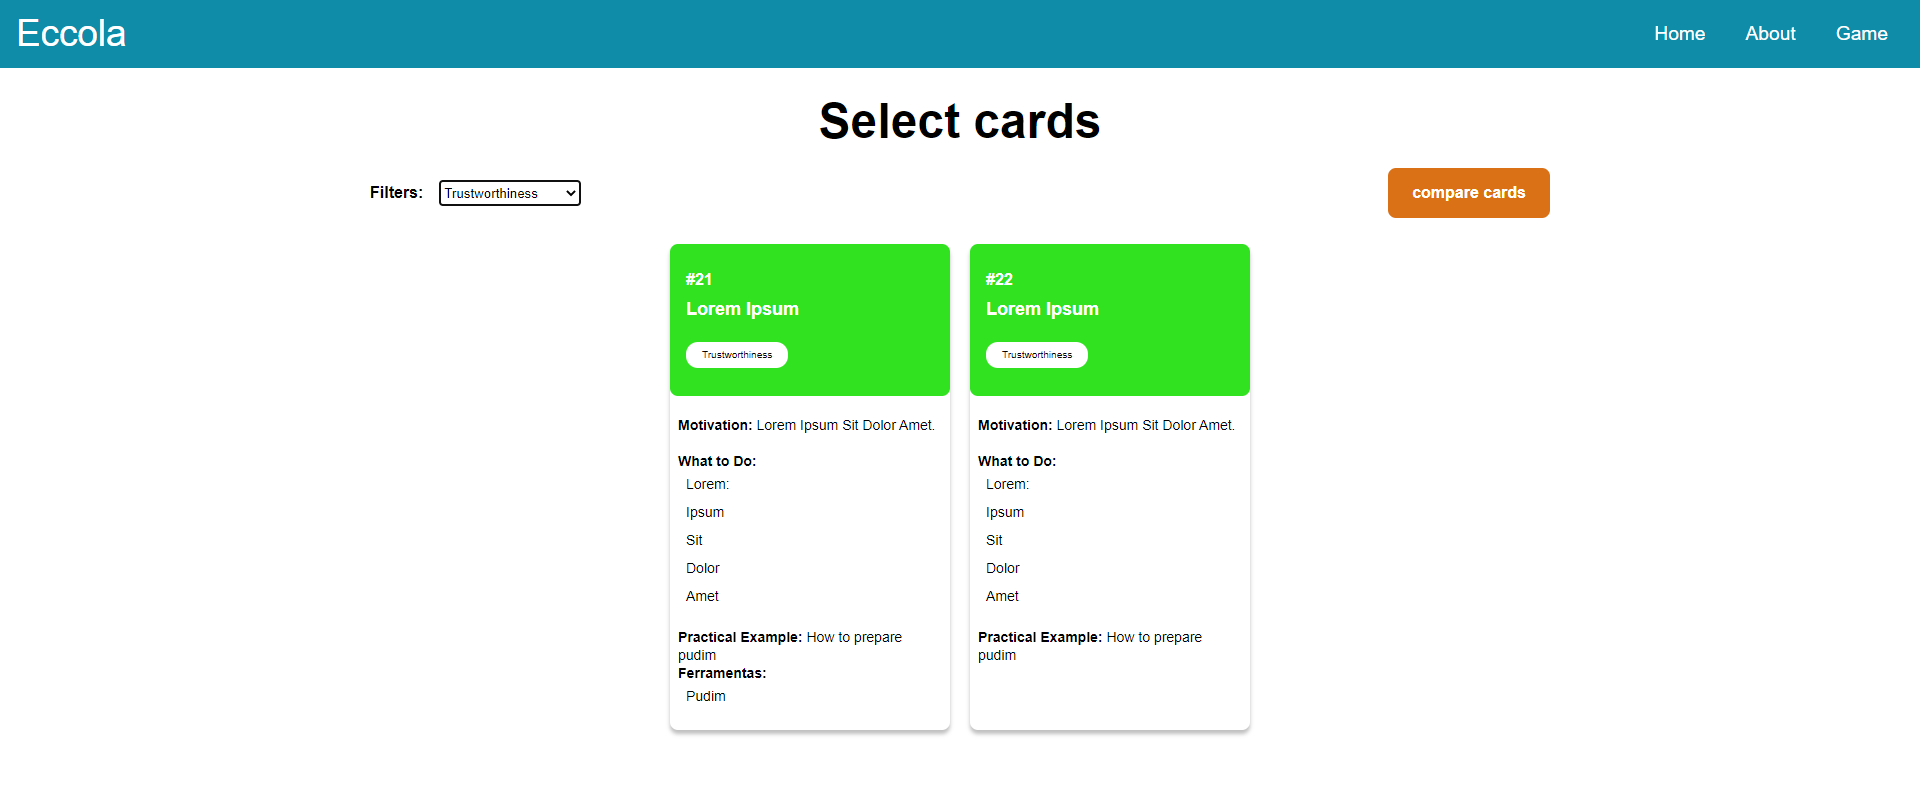
\includegraphics[width=\textwidth]{img/trustworthiness.png}
    \caption{Imagem do sistema com os \textit{cards Trustworthiness} criados.}
    \label{fig:trustworthiness}
\end{figure}

Para realizar a inserção destas informações dos \textit{cards}, basta colocar as informações conforme o modelo no snippet a seguir:

\begin{lstlisting}[language=JavaScript, caption=Informações novas inseridas nos cards]
const infosCards = [
{
    number: "21",
    type: "Trustworthiness",
    title: "Lorem Ipsum",
    motivation:
      "Lorem Ipsum Sit Dolor Amet.",
    whatToDo: [
      "Lorem:",
      "Ipsum",
      "Sit",
      "Dolor",
      "Amet",
    ],
    praticalExample: "How to prepare pudim",
    links: [
      {
        descricao: 'Pudim',
        link: 'http://www.pudim.com.br'
      },
    ]
  },

  {
    number: "22",
    type: "Trustworthiness",
    title: "Lorem Ipsum",
    motivation:
      "Lorem Ipsum Sit Dolor Amet.",
    whatToDo: [
      "Lorem:",
      "Ipsum",
      "Sit",
      "Dolor",
      "Amet",
    ],
    praticalExample: "How to prepare pudim",
    links: ""
  },
 ]
\end{lstlisting}

\subsection{Como editar um \textit{card} a classe já existente}
Com as informações descritas acima, caso haja algum card que não foi descrito conforme o requerido pelo usuário, só é necessário editar o arquivo \textit{infosCards.js}, conforme descrito anteriormente na seção anterior. O único requisito necessário é manter a ordem de acordo o tipo do \textit{card} que está na variável \textit{type}. Caso seja feita a inserção em um \textit{card} entre  duas classes já pré-existentes, tomar cuidado na numeração, uma vez que o sistema no estado atual não se encontra com auto-ordenação implantada. Logo, ao se adicionar um \textit{card} em classe já existente, não deixar de alterar a numeração no campo \textit{number} nos demais \textit{cards} consequentes.

\subsection{Como editar um \textit{card}}
Para realizar a edição de um \textit{card} já existente, somente é necessário seguir as instruções no \textit{snippet} 3.26, que mostra como adicionar as informações no arquivo \textit{infoCards.js}. Para tanto, somente é necessário um editor de texto simples (por exemplo, o Bloco de Notas, presente no \textit{Microsoft Windows} ou o VIM, presente em qualquer sistema operacional \textit{Linux}) e salvar, sem deixar de colocar as strings entre aspas e, ao terminar de escrever o que deseja, inserir um vírgula ao final. A inserção deste vírgula irá auxiliar inclusive se for preciso inserir novas informações no futuro sem quebrar o \textit{layout} do \textit{card}. 

Para fins de comparaçao entre o guia ECCOLA original e o ECCOLA modificado como neste exemplo, para ver as alterações realizadas basta acessar o link \url{https://oggvaldo.github.com/aiethicsguide}.

\section{Como obter o código-fonte do guia}
Para a obtenção do código-fonte do guia, este se encontra localizado no GitHub com o link \url{https://github.com/oggvaldo/aiethicsguide}. Para tanto, o usuário tem a opção ou de realizar um \textit{fork} do projeto, puxando e mantendo os arquivos no GitHub de uso do usuário ou baixando os arquivos clicando no botão \textit{Code} presente na página. Ao clicar no botão o próprio GitHub dá a opção de baixar os arquivos como um arquivo .zip ou realizar o clone via linha de comando usando o programa Git ou os programas GitHub Desktop ou GitHub CLI (que executa a mesma função que o Git, porém com códigos mais específicos para esta plataforma).

\begin{figure}[h!]
    \centering
    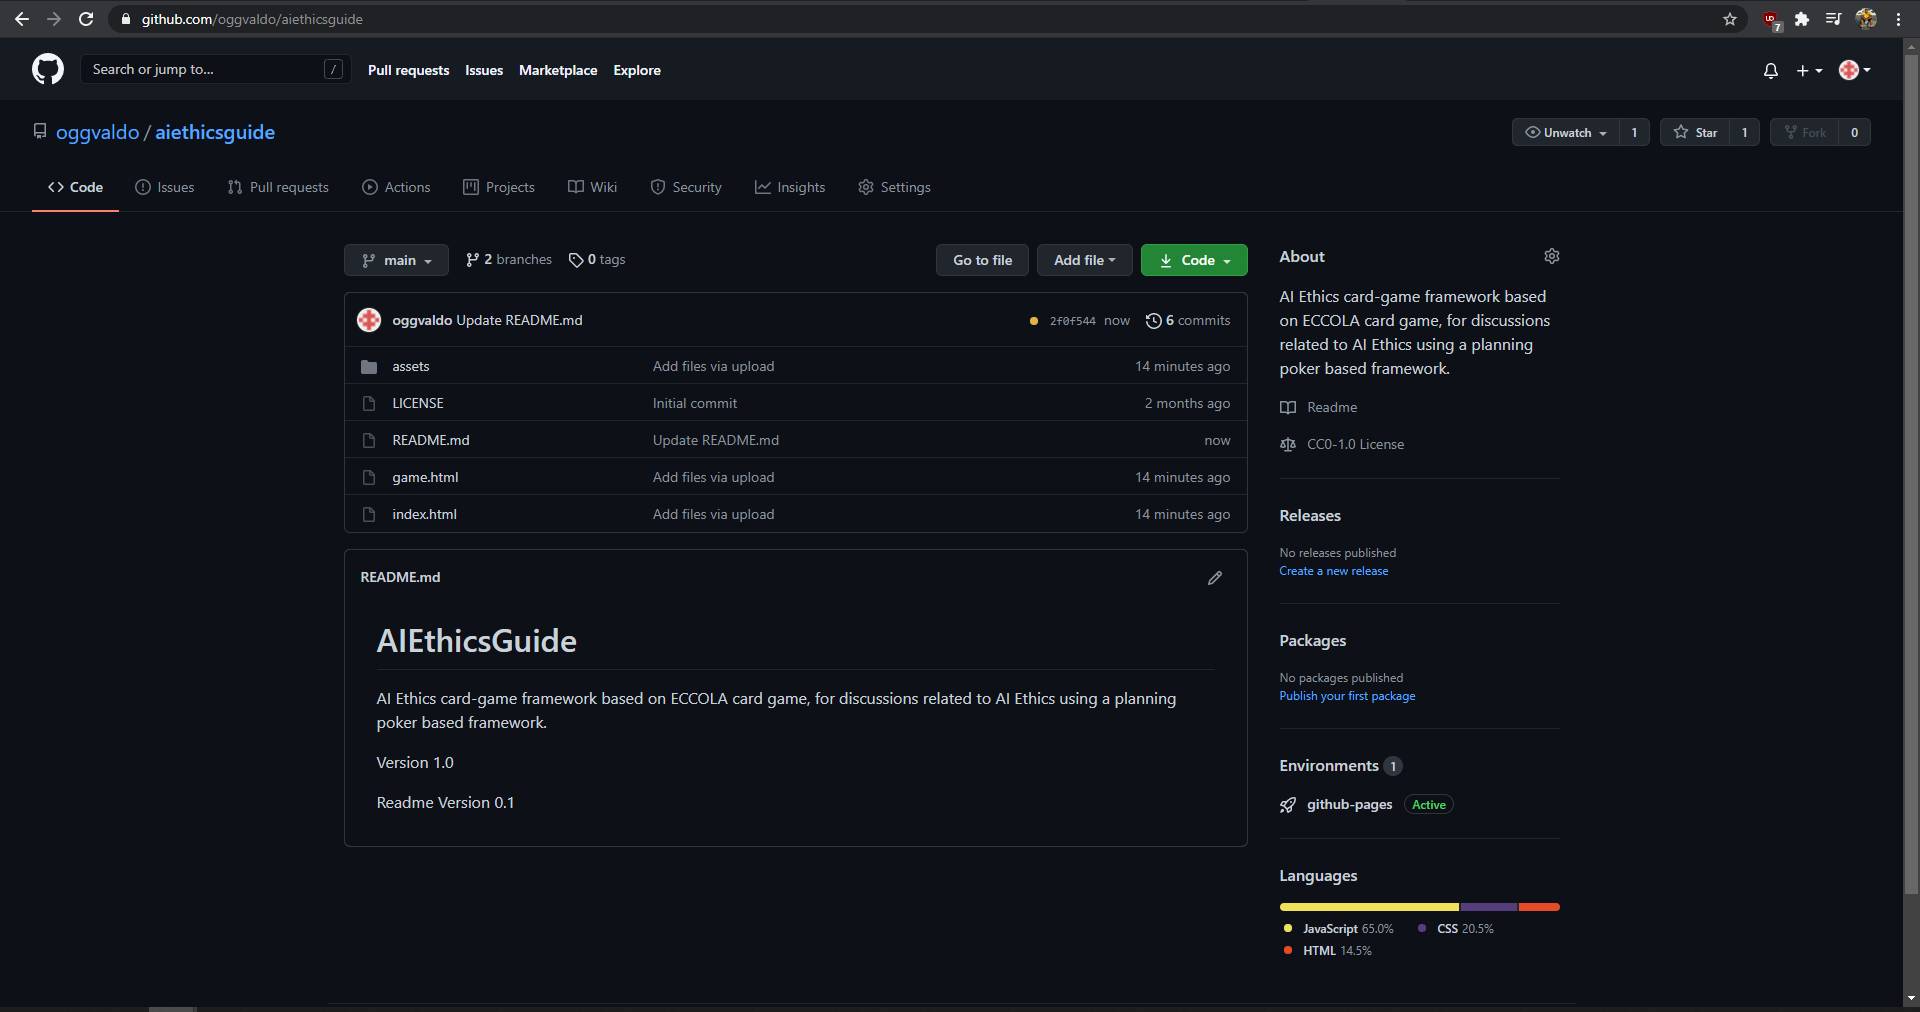
\includegraphics[width=\textwidth]{img/github.png}
    \caption{Imagem do github contendo os códigos-fontes.}
    \label{fig:github}
\end{figure}

\section{Síntese do Capítulo}
Foi apresentado neste Capítulo como se deu o desenvolvimento do sistema para o guia. Com a possibilidade de modularização, edição e simplicidade de uso, tanto para o usuário final -- que utiliza os cards --, como ao usuário que deseja inserir seus próprios princípios éticos de IA, este guia oferece aos usuários um meio favorável para a implementação de ética em IA em projetos que envolvem o desenvolvimento de sistemas baseados em IA. Vimos a necessidade do uso de JavaScript e \acrshort{CSS} para garantir o aspecto gráfico a este sistema baseado em \acrshort{HTML}, o que assim permite que ele seja ao mesmo tempo um WebApp simples e prático. Também foi apresentado a construção do sistem, com uma breve documentação do código-fonte, destacando os trechos mais importantes e como é realizada a edição de trechos do código para a inserção e edição de cards. Verificamos também algumas limitações do sistema, e como mitiga-los a fim de reduzir impactos gerados durante a etapa de inserção de novos princípios éticos, a serem empregados em versões futuras do guia.